%!TEX TS-program = xelatex
\documentclass[12pt, a4paper, oneside]{article}

\usepackage{amsmath,amsfonts,amssymb,amsthm,mathtools}  % пакеты для математики

\usepackage[english, russian]{babel} % выбор языка для документа
\usepackage[utf8]{inputenc} % задание utf8 кодировки исходного tex файла
\usepackage[X2,T2A]{fontenc}        % кодировка

\usepackage{fontspec}         % пакет для подгрузки шрифтов
\setmainfont{Linux Libertine O}   % задаёт основной шрифт документа

\usepackage{unicode-math}     % пакет для установки математического шрифта
\setmathfont[math-style=upright]{Neo Euler} % шрифт для математики

% Конкретный символ из конкретного шрифта
% \setmathfont[range=\int]{Neo Euler}

% Конкретный символ из конкретного шрифта
% \setmathfont[range=\int]{Neo Euler}

%%%%%%%%%% Работа с картинками %%%%%%%%%
\usepackage{graphicx}                  % Для вставки рисунков
\usepackage{graphics}
\graphicspath{{images/}{pictures/}}    % можно указать папки с картинками
\usepackage{wrapfig}                   % Обтекание рисунков и таблиц текстом

%%%%%%%%%%%%%%%%%%%%%%%% Графики и рисование %%%%%%%%%%%%%%%%%%%%%%%%%%%%%%%%%
\usepackage{tikz, pgfplots}  % язык для рисования графики из latex'a

%%%%%%%%%% Гиперссылки %%%%%%%%%%
\usepackage{xcolor}              % разные цвета

\usepackage{hyperref}
\hypersetup{
	unicode=true,           % позволяет использовать юникодные символы
	colorlinks=true,       	% true - цветные ссылки, false - ссылки в рамках
	urlcolor=blue,          % цвет ссылки на url
	linkcolor=red,          % внутренние ссылки
	citecolor=green,        % на библиографию
	pdfnewwindow=true,      % при щелчке в pdf на ссылку откроется новый pdf
	breaklinks              % если ссылка не умещается в одну строку, разбивать ли ее на две части?
}


\usepackage{todonotes} % для вставки в документ заметок о том, что осталось сделать
% \todo{Здесь надо коэффициенты исправить}
% \missingfigure{Здесь будет Последний день Помпеи}
% \listoftodos --- печатает все поставленные \todo'шки

\usepackage[paper=a4paper, top=20mm, bottom=15mm,left=20mm,right=15mm]{geometry}
\usepackage{indentfirst}       % установка отступа в первом абзаце главы

\usepackage{setspace}
\setstretch{1.15}  % Межстрочный интервал
\setlength{\parskip}{4mm}   % Расстояние между абзацами
% Разные длины в латехе https://en.wikibooks.org/wiki/LaTeX/Lengths


\usepackage{xcolor} % Enabling mixing colors and color's call by 'svgnames'

\definecolor{MyColor1}{rgb}{0.2,0.4,0.6} %mix personal color
\newcommand{\textb}{\color{Black} \usefont{OT1}{lmss}{m}{n}}
\newcommand{\blue}{\color{MyColor1} \usefont{OT1}{lmss}{m}{n}}
\newcommand{\blueb}{\color{MyColor1} \usefont{OT1}{lmss}{b}{n}}
\newcommand{\red}{\color{LightCoral} \usefont{OT1}{lmss}{m}{n}}
\newcommand{\green}{\color{Turquoise} \usefont{OT1}{lmss}{m}{n}}

\usepackage{titlesec}
\usepackage{sectsty}
%%%%%%%%%%%%%%%%%%%%%%%%
%set section/subsections HEADINGS font and color
\sectionfont{\color{MyColor1}}  % sets colour of sections
\subsectionfont{\color{MyColor1}}  % sets colour of sections

%set section enumerator to arabic number (see footnotes markings alternatives)
\renewcommand\thesection{\arabic{section}.} %define sections numbering
\renewcommand\thesubsection{\thesection\arabic{subsection}} %subsec.num.

%define new section style
\newcommand{\mysection}{
	\titleformat{\section} [runin] {\usefont{OT1}{lmss}{b}{n}\color{MyColor1}} 
	{\thesection} {3pt} {} } 


%	CAPTIONS
\usepackage{caption}
\usepackage{subcaption}
%%%%%%%%%%%%%%%%%%%%%%%%
\captionsetup[figure]{labelfont={color=Turquoise}}

\pagestyle{empty}


%%%%%%%%%% Свои команды %%%%%%%%%%
\usepackage{etoolbox}    % логические операторы для своих макросов

% Все свои команды лучше всего определять не по ходу текста, как это сделано в этом документе, а в преамбуле!

% Одно из применений - уничтожение какого-то куска текста!
\newbool{answers}
%\booltrue{answers}
\boolfalse{answers}

\usepackage{enumitem}
% бульпоинты в списках
\definecolor{myblue}{rgb}{0, 0.45, 0.70}
\newcommand*{\MyPoint}{\tikz \draw [baseline, fill=myblue,draw=blue] circle (2.5pt);}
\renewcommand{\labelitemi}{\MyPoint}

% расстояние в списках
\setlist[itemize]{parsep=0.4em,itemsep=0em,topsep=0ex}
\setlist[enumerate]{parsep=0.4em,itemsep=0em,topsep=0ex}

\begin{document}

%\section*{Самостоятельная работа номер 1. Вариант III}
%
%\textbf{Решите все задания. Все ответы должны быть обоснованы. Все решения должны быть чётко приведены для каждого пункта. Рисунки должны быть чёткими, понятными. Все лнии должны быть подписаны. Списывание карается обнулением баллов. Удачи!}
%
%\subsection*{[7] Задание 1}
%
%Примените метод $K$-means с $K=4$. В качестве начальных точек используйте $(0,2)$, $(0,1)$, $(-1,-3)$, $(-1,-2)$.	Опишите алгоритм выбора оптимального числа кластеров для $k-means$ (не надо это проделывать, просто опишите алгоритм).
%
%\begin{center}
%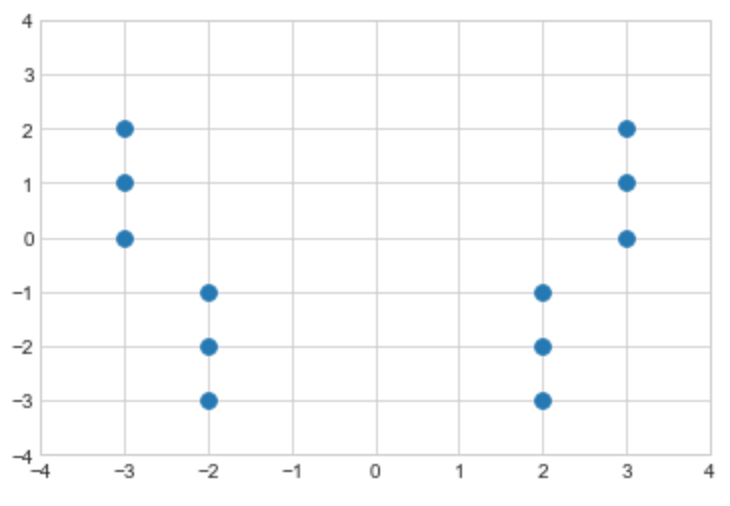
\includegraphics[scale=0.3]{knn_3.png}
%\end{center}
%
%
%\subsection*{[3] Задание 2}
%
%Обозначьте расположение центроидов и границ кластеров после применения метода K-means c $K=2$ на следущих данных: 
%
%\begin{minipage}[t]{0.66\textwidth}
%\begin{center}
%	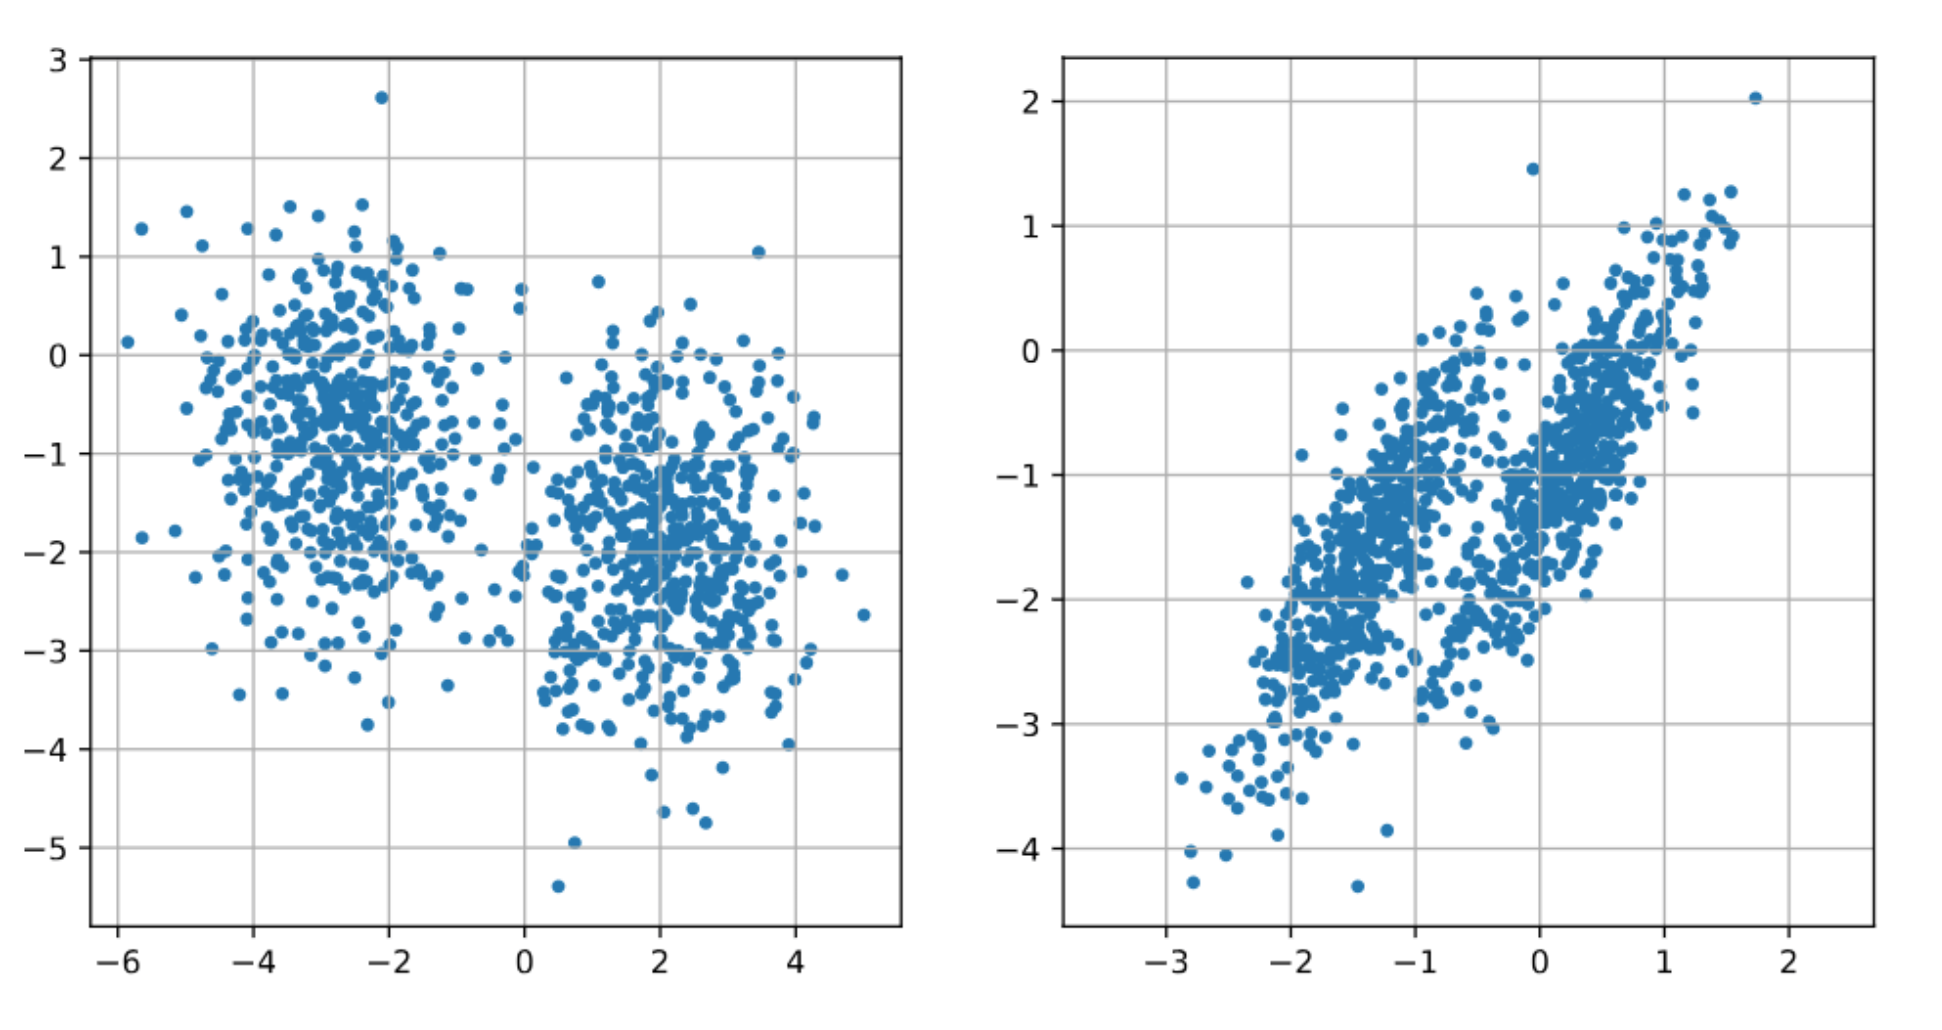
\includegraphics[scale=0.15]{clouds.png}
%\end{center}
%\end{minipage}
%\begin{minipage}[t]{0.33\textwidth}
%\begin{center}
%	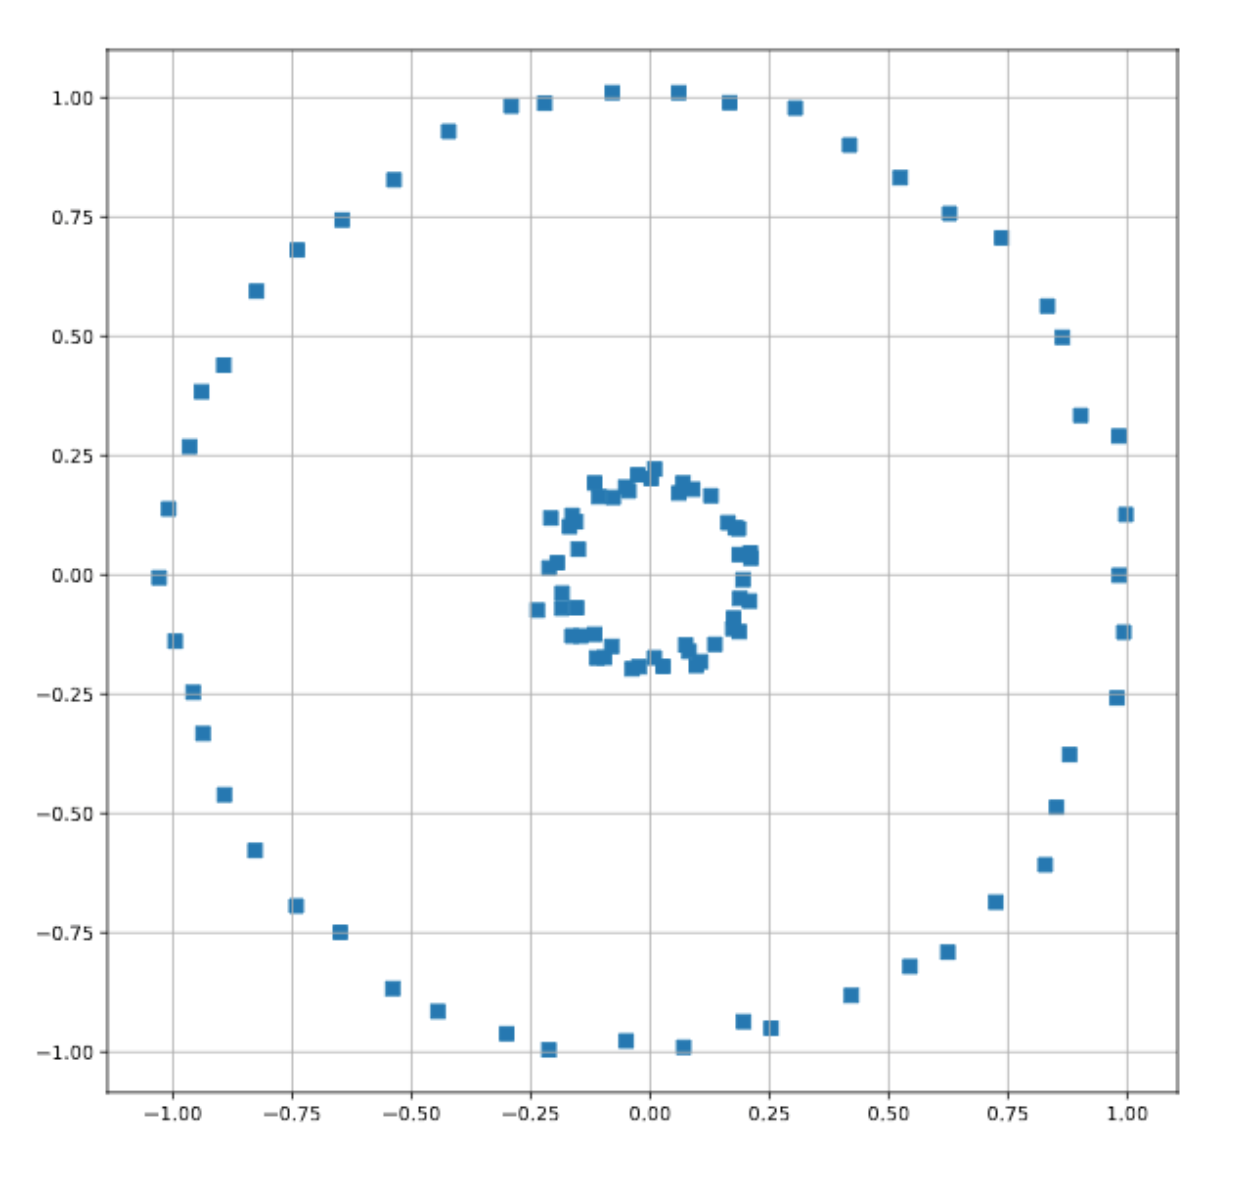
\includegraphics[scale=0.13]{circles.png}
%\end{center}
%\end{minipage}

%
%\newpage 


%\section*{Самостоятельная работа номер 2. Вариант III}
%
%\textbf{Решите все задания. Все ответы должны быть обоснованы. Все решения должны быть чётко приведены для каждого пункта. Рисунки должны быть чёткими, понятными. Все лнии должны быть подписаны. Списывание карается обнулением баллов. Удачи!}
%
%%\subsection*{[2.5] Задание 1 }
%%\begin{enumerate}
%%	
%%	\item  Мы стремимся переобучить любой алгоритм, так как в таком случае он хорошо запомнит выборку.
%%	
%%	\hspace{2cm} \textbf{Да}  \hspace{4cm} \textbf{Нет} 
%%	
%%	\item  Коэффициент силуэта используется, чтобы оценить успешность кластеризации и  расчитывается как доля правильно предсказанных кластеров.
%%	
%%	\hspace{2cm} \textbf{Да}  \hspace{4cm} \textbf{Нет} 
%%	
%%	\item  Качество модели может сильно зависеть от того как именно мы поделили. выборку на трэйн и тест. Чтобы сгладить этот эффект используют кросс-валидацию.
%%	
%%	\hspace{2cm} \textbf{Да}  \hspace{4cm} \textbf{Нет} 
%%	
%%	\item  Метод ближайших соседей никогда не переобучается. 
%%	
%%	\hspace{2cm} \textbf{Да}  \hspace{4cm} \textbf{Нет} 
%%	
%%	\item  Для задачи кластеризации, в отличие от задачи классификации, мы заранее знаем правильные ответы. 
%%	
%%	\hspace{2cm} \textbf{Да}  \hspace{4cm} \textbf{Нет} 
%%	
%%	\item  	Хорошо, что не было вопросов про случайный лес.
%%	
%%	\hspace{2cm} \textbf{Да}  \hspace{4cm} \textbf{Нет} 
%%
%%\end{enumerate}
%
%\subsection*{[2] Задание 1 }
%
%Дайте краткий (не более двух предложений) ответ на следущие вопросы: 
%
%\begin{enumerate}
%	\item  Зачем разделять выборку на тренировочную и тестовую? 
%	
%	\item Чем задача обучения с учителем отличается от задачи обучения без учителя? 
%	
%	\item Что такое переобучение? 
%	
%	\item Что такое кросс-валидация? Зачем её придумали, если выборку можно просто разделить на тренировочную и тестовую. 
%	
%	\item Чем knn отличается от k-means? 
%\end{enumerate}
%
%
%\subsection*{[6] Задание 2}
%
%Арчибальд решает самостоятельную работу номер 2 по машинному обучению. Он подглядел у Анфисы переменную $y$ --- ответы на вопросы теста. А ещё он посчитал количество строк, которое анфиса написала на бумаге для того, чтобы этот ответ получить. Пятое задание подглядеть не получилось.  Арчибальд хочет по-быстрому оценить решающее дерево и спрогнозировать ответ на пятое задание. 
%
%\begin{center}
%	\begin{tabular}{cc}
%		$y_i$ & $x_i$ \\
%		\hline
%		да & $1$ \\
%		нет & $3$ \\
%		да & $4$ \\
%		нет& $6$ \\
%	\end{tabular}
%\end{center}
%
%Дерево строится до идеальной классификации. Критерий деления узла на два — минимизация числа допущенных ошибок.  Правило прогнозирования в каждой вершине: в качестве прогноза выдаем тот класс, представителей которого в вершине больше.  
%
%По прикидкам Арчибальда для решения пятого задания нужно написать $5$ строчек. Какой ответ надо дать на него? 
%
%%На плоскости расположены колонии рыжих и чёрных муравьёв. Рыжих колоний три и они имеют координаты $(-1, 1)$, $(1, -1)$ и $(1, 1)$. Чёрных колоний одна и она имеет координаты $(0, 0)$.
%%
%%\begin{enumerate}
%%\item Поделите плоскость на «зоны влияния» рыжих и чёрных используя метод одного и трёх ближайших соседей.
%%
%%\item С помощью кросс-валидации с выкидыванием отдельных наблюдений выберите оптимальное число соседей $k$ перебрав $k \in \{1, 3 \}$. Целевой функцией является количество несовпадающих прогнозов.
%%\end{enumerate}
%
%\newpage
%
%\subsection*{[1.5] Задание 3}
%
%Объясните мемас: 
%
%\begin{center}
%	
\includegraphics[scale=0.3]{memes2.jpg}
%\end{center}


%\newpage 


%\section*{Самостоятельная работа номер 3. Вариант I}
%
%\textbf{Решите все задания. Все ответы должны быть обоснованы. Все решения должны быть чётко приведены для каждого пункта. Рисунки должны быть чёткими, понятными. Все лнии должны быть подписаны. Списывание карается обнулением баллов. Удачи!}
%
%\subsection*{[3] Задание 1 }
%
%Драгомир пытается предсказать продажи видео-игр.  Для моделирования он использует две переменные: $x_1$ - возраст игры, $x_2$ - на кого она ориентирована. Если на мужчин, $x_2=1$, если на женщин, $x_2=0$. Целевая переменная $y$ - сумма продаж. Драгомир оценил линейную регрессию: 
%
%$$ y = 1000 - 100 \cdot  x_1 + 200 \cdot  x_2.$$
%
%Проинтерпретируйте полученные коэффициенты.  Предположим, что мы выпускаем на рынок свежую игру для женщин. Спрогнозируйте наши продажи. 
%
%
%\subsection*{[5] Задание 2}
%
%Маше $13$ лет. Всю свою жизнь она занималась коллекционированием моделей.  Вчера она пообщалась с Мишей. Он тоже коллекционер. Он спросил у неё, какое у её моделей качество? Маша не смогла ответить и решила проверить его. У неё есть три наблюдения $y_i$. Она для каждого построила прогнозы. Найдите для её прогнозов MAE и RMSE.
%
%\begin{center}
%	\begin{tabular}{c|c|c|c}
%		$y_i$ &  1 & 2 & 3 \\
%		\hline
%		Нейросеть & 2 & 3 & 1  \\
%		Регрессия &  2 & 3 & 4 \\
%		Лес & 1 & 1 & 1 \\
%	\end{tabular}
%\end{center}
%
%
%\subsection*{[2] Задание 3}
%
%Объясните мемас: 
%
%\begin{center}
%	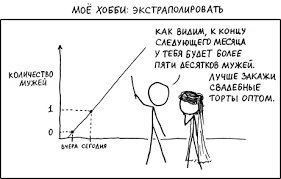
\includegraphics[scale=0.7]{memes.png}
%\end{center}

%\newpage 

\section*{Самостоятельная работа номер 4. Вариант I}

\textbf{Решите все задания. Все ответы должны быть обоснованы. Все решения должны быть чётко приведены для каждого пункта. Рисунки должны быть чёткими, понятными. Все лнии должны быть подписаны. Списывание карается обнулением баллов. Удачи!}

\subsection*{[10] Задание 1 }

Всю свою жизнь Филипп был бездельником и сидел на шее у родителей. Но наконец ему улыбнулась удача и его взяли на работу аналитиком. Теперь он борется со всем плохим и за всё хорошее внутри большой рекомендательной системы. 

Когда пользователь рекомендательной системы встречает в статьях матерную брань, он очень сильно расстраивается. Из-за этого одной из задач Филиппа является воспитание модели, которая могла бы дать бой нецензурщине. 

Филипп оценил модель и получил на тестовой выборке следущие прогнозы вероятностей: 

\begin{center}
	\begin{tabular}{c|c}
		$y_i$ & $b_i$ \\
		\hline
		$1$  & $0.99$ \\
		$1$ & $0.8$ \\
		$0$ & $0.77$ \\
		$1$ & $0.55$ \\
		$0$  & $0.55$ \\
		$0$ & $0.4$ \\
		$1$ & $0.3$ \\
		$0$ & $0.2$ \\
	\end{tabular}
\end{center}


В первой колонке стоит $1$, если статья была матерной и стоит $0$, если статья оказалась обычной. Во второй колонке стоит вероятность того, что статья окажется матерной, предсказанная моделью. Филипп размышляет над тем какой бы для модели выбрать порог: $0.5$, $0.7$ или $0.9$. 

\begin{enumerate}
	\item[(4)] Найдите для каждого порога precision и recall. Какой порог вы бы порекомендовали поставить? Обоснуйте ответ.
	
	\item[(4)] Что такое roc-auc? Зачем изобрели эту метрику? Посчитайте её.
	
	\item[(2)]  Что такое accuracy? Чем плоха эта метрика качества? Предложите конкретный численный пример, на котором эта метрика плохо себя показывает.
	
\end{enumerate}



%\newpage 


%\section*{Долгожданный Кекс}
%
%\subsection*{Постановка задачи} 
%
%<<Волшебная лавка мистера Оливандера>> --- крупнейший онлайн-магазин волшебной атрибутики, недоступной для Маглов.  Её владелец, мистер Оливандер, недавно услышал о том, какую магию с его онлайн-ритейлом могут сотворить маркетологи, обученные анализу данных. Именно поэтому он пришёл за помощью к вам. 
%
%Мистер Оливандер довольно продвинутый маг. Он знает, что жизненный цикл клиента удобно изображать с помощью <<воронки>>, описывающей движение человека по процессу покупки.  Он понимает, что иногда бывает так, что клиенты приуныли. Обычно это происходит при переходе с одного шага воронки на другой. 
%
%Например, из 100 человек, увидевших рекламу, только 20 кликнут на неё и перейдут на сайт. Из перешедших на сайт только половина добавит товар в корзину, из добавивших товар в корзину, только четверть совершит покупку. На каждом этапе по каким-то причинам клиенты отваливаются. И это не очень круто. Увеличивая количество клиентов на каком-либо уровне воронки, мы автоматически увеличиваем результирующий объем продаж. Для этого надо как-то воздействовать на клиентов, но как именно непонятно. 
%
%Мистер Оливандер очень хочет избежать состояния клиентов <<что-то приуныли>> и повысить ключевые показатели своего бизнеса. Что за ключевые показатели, он толком не определился и надеется на ваши дельные советы. Вам необходимо сделать следущие вещи: 
%
%\begin{enumerate}
%	\item Определить как выглядит воронка магического онлайн-ритейла и понять где именно при проходе по ней могут отваливаться клиенты. 
%	
%	\item Определиться, на какие ключевые показатели, то есть метрики, необходимо ориентироваться на каждом этапе воронки, чтобы понимать улучшилась ситуация или ухудшилась. Для каждого этапа сформулируйте пул из нескольких метрик.
%	
%	\item Понять как с помощью машинного обучения можно <<улучшить>> прохождение человека по воронке, определиться какие данные для этого использовать, откуда их взять. 
%\end{enumerate}
%
%
%\subsection*{Правила игры и оценивание} 
%
%Кекс делается в группах по три человека. За сделанную работу группе выставляется $30$ баллов. Баллы нужно будет поделить между членами группы самостоятельно. 
%
%Например, в группе работали Гермиона, Гарри и Рон. В итоге они получили $25$ баллов. Гермиона работала больше всех, команда решает отдать ей $15$ баллов. Гарри работал похуже, он получает $10$ баллов. Рон --- балбес, который ничего, по мнению команды, не делал. Он баллы не получает. 
%
%Ваша итоговая оценка зависит от того, насколько глубоко проработана задача, насколько чётко обоснован каждый этап работы, каждая метрика.  Оцениваться будут следущие пойнты: 
%
%\begin{itemize}
%	\item Продуманность воронки, обоснованность каждой её части. 
%	\item Продуманность и обоснованность системы метрик для монтиринга прохода по воронке. 	
%	\item Адекватность данных, выбранных для оценивания модели.
%	\item Обоснование выбранных переменных. Чётко объясните почему вы выбрали в качестве целевой переменной именно то, что вы выбрали. Постарайтесь объяснить как именно ваша модель поможет достичь желаемого результата. 
%\end{itemize}
%
%Обратите внимание, что от вас никто не требует описывать как вы делаете кросс-валидацию, дробите выборку и как вообще работает метод ближайшего соседа. Подразумевается, что это очевидно. Нас интересует именно ваше понимание того, как состыкуются между собой бизнес и машинное обучение, а не знание алгоритмов. Жизнь первична, технические детали вторичны. Не забывайте об этом. 
%
%\subsection*{Куда сдавать и когда сдавать}
%
%На кекс у вас есть текущий семинар. Сгенерируйте в рамках своей группы его решение и тезисно оформите его на бумаге от руки так, чтобы проверяющий понял что вы имеете в виду и не сошёл с ума при проверке работы. Не забудьте подписать работы всеми тремя фамилиями и сдать их. 

\end{document}



